% Point spreads for two runs of blah

\begin{figure}
\center

\begin{subfigure}[b]{0.45\textwidth}
	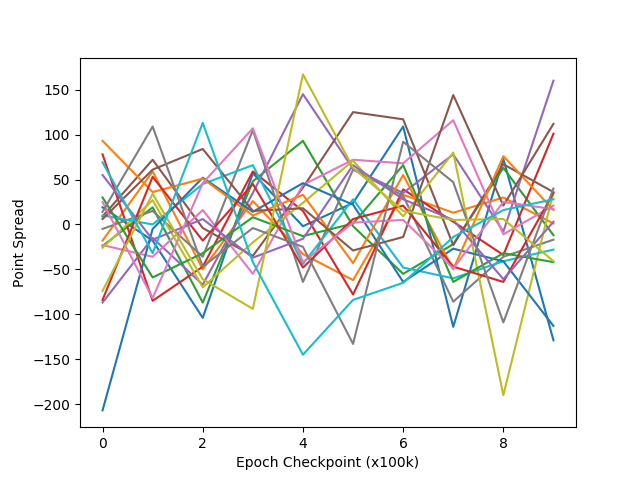
\includegraphics[width=\linewidth]{images/findings/round2/spreads_self-v-prev_winner.png}
	\caption{An agent plays against previous iterations of itself.}
	\label{fig:r2-spreads-winner-a}
\end{subfigure}
~
\begin{subfigure}[b]{0.45\textwidth}
	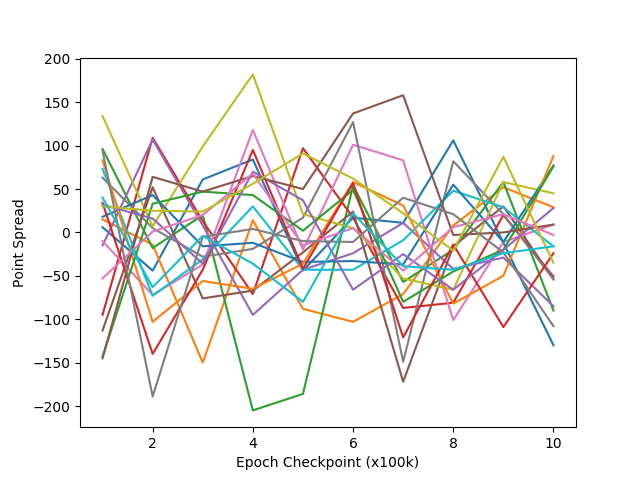
\includegraphics[width=\linewidth]{images/findings/round2/spreads_rand-v-fut_winner.png}
	\caption{A random agent plays against later, more learned agents.}
	\label{fig:r2-spreads-winner-b}
\end{subfigure}

\caption{
	Point spreads across multiple 9-game tournaments for an agent in the
	winners' bracket of Round 2.
	Note that since the winners' bracket uses an agent with prior training,
	the total epochs elapsed is one million more than displayed.
}
\label{fig:r2-spreads-winner}
\end{figure}
